\documentclass[tikz,border=2pt,11pt]{standalone}
\usetikzlibrary{arrows.meta}
\usepackage{amsmath}
\usepackage{amssymb}
\usepackage{tikz}
\usepackage{xcolor}
\renewcommand{\mapsto}{
  \BeginAccSupp{pdfliteral=direct,method=hex,unicode,ActualText=21A6}
  \KSOriginalMapsto\EndAccSupp{pdfliteral=direct}}
\renewcommand{\hookrightarrow}{
  \BeginAccSupp{pdfliteral=direct,method=hex,unicode,ActualText=21AA}
  \KSOriginalHookrightarrow\EndAccSupp{pdfliteral=direct}}
\renewcommand{\ne}{
  \BeginAccSupp{pdfliteral=direct,method=hex,unicode,ActualText=2260}
  \KSOriginalNe\EndAccSupp{pdfliteral=direct}}
\renewcommand{\notin}{
  \BeginAccSupp{pdfliteral=direct,method=hex,unicode,ActualText=2209}
  \KSOriginalNotin\EndAccSupp{pdfliteral=direct}}
\newcommand{\R}{\mathbf R}
\newcommand{\C}{\mathbf C}
\newcommand{\N}{\mathbf N}
\newcommand{\Z}{\mathbf Z}
\newcommand{\cH}{\mathcal H}
\newcommand{\cK}{\mathcal K}
\newcommand{\cD}{\mathcal D}
\newcommand{\cB}{\mathcal B}
\DeclareMathOperator{\id}{id}
\DeclareMathOperator{\Tr}{Tr}
\DeclareMathOperator{\Ran}{Ran}
\DeclareMathOperator{\Dom}{Dom}
\DeclareMathOperator{\supp}{supp}
\DeclareMathOperator{\Var}{Var}
\DeclareMathOperator{\diag}{diag}
\DeclareMathOperator*{\essinf}{ess\,inf}
\DeclareMathOperator*{\esssup}{ess\,sup}
\DeclareMathOperator{\sgn}{sgn}
\begin{document}
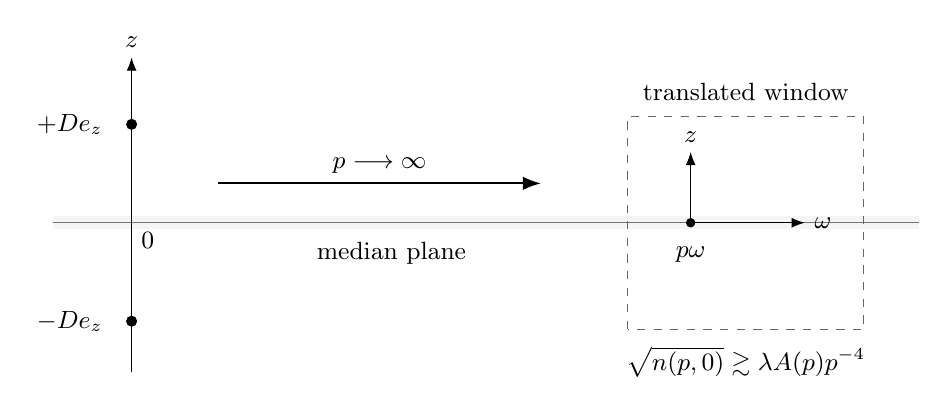
\begin{tikzpicture}[x=1cm,y=1cm,>=Latex,font=\small]
  \fill[black!4] (-1,-0.08) rectangle (10,0.08);
  \draw[black!55] (-1,0) -- (10,0);
  \draw[->] (0,-1.9) -- (0,2.1) node[above] {$z$};
  \fill (0,1.25) circle (2pt) node[left=7pt] {$+De_z$};
  \fill (0,-1.25) circle (2pt) node[left=7pt] {$-De_z$};
  \node[below right] at (0,0) {$0$};
  \node[below] at (3.3,-0.12) {median plane};
  \draw[->,thick] (1.1,0.5) -- (5.2,0.5)
    node[midway,above] {$p\longrightarrow\infty$};
  \draw[dashed,black!60] (6.3,-1.35) rectangle (9.3,1.35);
  \fill (7.1,0) circle (1.7pt) node[below=5pt] {$p\omega$};
  \draw[->] (7.1,0) -- (8.55,0) node[right] {$\omega$};
  \draw[->] (7.1,0) -- (7.1,0.9) node[above] {$z$};
  \node[above] at (7.8,1.43) {translated window};
  \node[below] at (7.8,-1.45) {$\sqrt{n(p,0)}\gtrsim\lambda A(p)p^{-4}$};
\end{tikzpicture}
\end{document}
